
% \titlegraphic{\hfill\includegraphics[height=1.5cm]{logo.pdf}}

\documentclass[xcolor=pdftex,dvipsnames,table,numbers,hyperref={pdfpagelabels=false},compress]{beamer}
%\usepackage{requiredPackage}
\usepackage{amsmath}
\usepackage{graphicx}
\usepackage{amsfonts}
\usepackage{amssymb}

\usepackage{tabularx}
\usepackage{epstopdf}
\usepackage{overpic}
\usepackage{url}
\usepackage{calrsfs}
\usepackage{mathrsfs}
\usepackage{epsfig}
\usepackage{cancel}
\usepackage{changepage}

\usepackage{tikz}
\usepackage[customcolors]{hf-tikz} 

\usepackage{lmodern}
%\usepackage{mystyle}
\usepackage{subfig}
\usepackage{pifont}
\usepackage{tabu}
\usepackage{xcolor}
\usepackage{algorithm}
\usepackage{algpseudocode}
%\usepackage{enumitem}
\usepackage{remreset}
\usepackage{etoolbox}
\usepackage{comment} % end and begin comment
%\usepackage{dtklogos} 
\usepackage{listings}
\lstset{breaklines=true} 

\newcommand{\gline}{\textcolor{gray}{\hline}}
\newcommand{\cmark}{\ding{51}}%
\newcommand{\xmark}{\ding{55}}%
\newcommand{\gcheck}{\textcolor{blue}{\Large \cmark}}
\newcommand{\rcross}{\textcolor{red}{\Large \xmark}}
\newcommand{\tkt}{\tilde{K}_\theta}
\newcommand{\kt}{K_\theta}
\newcommand{\ind}{\overset{ind}{\sim}}
\newcommand{\plim}{\overset{p}{\rightarrow}}
\newcommand{\cx}{\frac {X'X}n}
\newcommand{\cz}{\frac {Z'Z}n}
\newcommand{\ccz}{\frac {Z'Z}n - \Sigma_A}
\newcommand{\czy}{\frac {Z'y}n}
\newcommand{\cyz}{\frac {y'Z}n}
\newcommand{\cxy}{\frac {X'y}n}
\newcommand{\cyx}{\frac {y'X}n}
\newcommand{\myitem}{\vskip3mm \item}

\newcommand{\calS}{{\cal S}}
\newcommand{\calA}{{\cal A}}
\newcommand{\calK}{{\cal K}}
\newcommand{\calX}{{\cal X}}
\newcommand{\calD}{{\cal D}}
\newcommand{\calG}{{\cal G}}
\newcommand{\calT}{{\cal T}}
\newcommand{\calU}{{\cal U}}
\newcommand{\calR}{{\cal R}}
\newcommand{\tp}{\tilde{p}}
\newcommand{\tildebC}{\tilde{\bC}}
\newcommand{\calL}{{\cal L}}

\newcommand{\blam}{ \mbox{\boldmath $ \lambda $} }
\newcommand{\bet}{ \mbox{\boldmath $ \eta $} }
\newcommand{\bome}{ \mbox{\boldmath $ \omega $} }
\newcommand{\bbet}{ \mbox{\boldmath $ \beta $} }
\newcommand{\bbeta}{ \mbox{\boldmath $ \beta $} }
\newcommand{\balph}{ \mbox{\boldmath $ \alpha $} }
\newcommand{\balpha}{ \mbox{\boldmath $ \alpha $} }
\newcommand{\bphi}{ \mbox{\boldmath $\phi$}}
\newcommand{\bzeta}{ \mbox{\boldmath $\zeta$}}
\newcommand{\bkap}{ \mbox{\boldmath $\kappa$}}
\newcommand{\bkappa}{ \mbox{\boldmath $\kappa$}}
\newcommand{\beps}{ \mbox{\boldmath $\epsilon$}}
\newcommand{\bepsilon}{ \mbox{\boldmath $\epsilon$}}
\newcommand{\bthet}{ \mbox{\boldmath $ \theta $} }
\newcommand{\btheta}{ \mbox{\boldmath $ \theta $} }
\newcommand{\blambda}{ \mbox{\boldmath $ \lambda $} }
\newcommand{\bnu}{ \mbox{\boldmath $\nu$} }
\newcommand{\bmu}{ \mbox{\boldmath $\mu$} }
\newcommand{\bGam}{ \mbox{\boldmath $\Gamma$} }
\newcommand{\bSig}{ \mbox{\boldmath $\Sigma$} }
\newcommand{\bSigma}{ \mbox{\boldmath $\Sigma$} }
\newcommand{\bPhi}{ \mbox{\boldmath $\Phi$} }
\newcommand{\bThet}{ \mbox{\boldmath $\Theta$} }
\newcommand{\bTheta}{ \mbox{\boldmath $\Theta$} }
\newcommand{\bDel}{ \mbox{\boldmath $\Delta$} }
\newcommand{\bDelta}{ \mbox{\boldmath $\Delta$} }
\newcommand{\bnabla}{ \mbox{\boldmath $\nabla$} }
\newcommand{\bLam}{ \mbox{\boldmath $\Lambda$} }
\newcommand{\bLambda}{ \mbox{\boldmath $\Lambda$} }
\newcommand{\bgam}{ \mbox{\boldmath $\gamma$} }
\newcommand{\bgamma}{ \mbox{\boldmath $\gamma$} }
\newcommand{\brho}{ \mbox{\boldmath $\rho$} }
\newcommand{\bdel}{ \mbox{\boldmath $\delta$} }
\newcommand{\bdelta}{ \mbox{\boldmath $\delta$} }
\newcommand{\sis}{\sigma^2}
\newcommand{\bOmega}{\mbox{\boldmath $\Omega$} }
\newcommand{\bPsi}{ {\boldsymbol \Psi} }
\newcommand{\btkt}{\boldsymbol{\tilde{K}}_\theta}
\newcommand{\pg}{P{\'o}lya-Gamma }

\newcommand{\bzero}{\textbf{0}}
\newcommand{\bones}{\textbf{1}}
\newcommand{\ba}{\textbf{a}}
\newcommand{\bb}{\textbf{b}}
\newcommand{\bB}{\textbf{B}}
%\newcommand{\bA}{\textbf{A}}
\newcommand{\bc}{\textbf{c}}
\newcommand{\bC}{\textbf{C}}
\newcommand{\bA}{\textbf{A}}
\newcommand{\bd}{\textbf{d}}
\newcommand{\bD}{\textbf{D}}
\newcommand{\be}{\textbf{e}}
\newcommand{\bE}{\textbf{E}}
\newcommand{\bk}{\textbf{k}}
\newcommand{\bK}{\textbf{K}}
\newcommand{\bh}{\textbf{h}}
\newcommand{\bs}{\textbf{s}}
\newcommand{\bS}{\textbf{S}}
\newcommand{\bH}{\textbf{H}}
\newcommand{\bI}{\textbf{I}}
\newcommand{\bt}{\textbf{t}}
\newcommand{\bu}{\textbf{u}}
\newcommand{\bv}{\textbf{v}}
\newcommand{\bw}{\textbf{w}}
\newcommand{\bW}{\textbf{W}}
\newcommand{\bx}{\textbf{x}}
\newcommand{\bX}{\textbf{X}}
\newcommand{\by}{\textbf{y}}
\newcommand{\bY}{\textbf{Y}}
\newcommand{\bz}{\textbf{z}}
\newcommand{\bZ}{\textbf{Z}}
\newcommand{\bL}{\textbf{L}}
\newcommand{\br}{\textbf{r}}
\newcommand{\bR}{\textbf{R}}
\newcommand{\bm}{\textbf{m}}
\newcommand{\bM}{\textbf{M}}
\newcommand{\given}{\,|\,}
\newcommand{\T}{\top}
\newcommand{\bV}{\textbf{V}}
\newcommand{\bJ}{\textbf{J}}
\newcommand{\blue}[1]{{\color{RoyalBlue!90} #1}}
\newcommand{\red}[1]{{\color{Red} #1}}
\newcommand{\green}[1]{{\color{Green} #1}}
\newcommand{\orange}[1]{{\color{Orange} #1}}
\newcommand{\titl}[1]{{\begin{large}\begin{center}#1\end{center}\end{large}}}

\newcommand{\tildea}{\tilde{a}}
\newcommand{\tildeba}{\tilde{\ba}}
\newcommand{\tildebv}{\tilde{\bv}}
\newcommand{\tildev}{\tilde{v}}
\newcommand{\tildeA}{\tilde{A}}
\newcommand{\tildeC}{\tilde{C}}
\newcommand{\tildeK}{\tilde{K}}
\newcommand{\tildew}{\tilde{w}}
\newcommand{\tildeu}{\tilde{u}}
\newcommand{\tildebw}{\tilde{\bw}}
\newcommand{\tildeeps}{\tilde{\epsilon}}
\newcommand{\tildebeps}{\tilde{\bepsilon}}
\newcommand{\eps}{\epsilon}
\newcommand{\sigs}{\sigma^2}
\newcommand{\taus}{\tau^2}
\newcommand{\iid}{\stackrel{\mathrm{iid}}{\sim}}

%\newcommand{\calS}{{\cal S}}
\newcommand{\calC}{{\cal C}}

%\documentclass[10pt]{beamer}

\usetheme{metropolis}
\usepackage{appendixnumberbeamer}

\usepackage{booktabs}
\usepackage[scale=2]{ccicons}

\usepackage{pgfplots}
\usepgfplotslibrary{dateplot}

\usepackage{xspace}
\newcommand{\themename}{\textbf{\textsc{metropolis}}\xspace}

\makeatletter
\@addtoreset{subfigure}{framenumber}% subfigure counter resets every frame
\makeatother

\makeatletter
\@addtoreset{figure}{framenumber}% subfigure counter resets every frame
\makeatother

\setbeamertemplate{caption}{\raggedright\insertcaption\par}
\captionsetup[subfigure]{labelformat=empty}


\title[]{Modeling non-Gaussian spatial data}
\author{Jeffrey Doser$^1$ \& Andrew Finley$^2$}
	
\institute{
\begin{tiny}$^1$Department of Integrative Biology, Michigan State University.\\
$^2$Department of Forestry, Michigan State University.\end{tiny}
}

\date{May 15, 2023}


\begin{document}

\maketitle

\begin{frame}{Non-Gaussian spatial data}

\begin{itemize}
	\item Often data sets preclude Gaussian modeling: $y(\bs)$ may not even be continuous
        \item Examples: 
             \begin{itemize}
		     \item Binary: presence or absence of a species at location s.
                     \item Count: abundance of a species at location s.
                     \item Categorical: counts of trees by size class at location s.  
             \end{itemize}
     \item Replace Gaussian likelihood by exponential family member (Diggle, Tawn, and Moyeed (1998)).
\end{itemize}
\end{frame}
 

\begin{frame}{Hierarchical Bayesian approach}
     \begin{itemize}
	     \item \textbf{First stage}: $y(\bs_i)$ are conditionally independent given
		     $\bbeta$ and $\text{w}(\bs_i)$. Here we use a canonical link function, say $g(E[y(\bs_i)]) = \eta(\bs_i) =\bx(\bs_i)'\bbeta+\text{w}(\bs_i)$. \pause
	     \item \textbf{Second stage}: Model $\text{w}(\bs_i)$ as a Gaussian process:
		     $$ \bw \sim N(\bzero,\sigma^2\bR(\phi))$$ \pause
	     \item \textbf{Third stage}: Priors and hyperpriors.
     \end{itemize}

\end{frame}

\begin{frame}{MCMC sampling for spatial GLMMs}
     \begin{itemize}
	     \item Additional GLMM flexibility comes at a computational cost: lose conjugacy of $\bbeta, \bw$
	     \item Requires more Metroplis steps. Particularly costly for $\bw$
	     \item Practical consequence: slower, less efficient algorithms
	     \item Prediction and interpolation proceed as with the Gaussian case
     \end{itemize}
\end{frame}

\begin{frame}{\pg data augmentation}
    \begin{itemize}
	    \item General approach for Bayesian (spatial) logistic regression that yields conjugate updates of $\bbeta$ (and $\bw$) \pause
	    \item Introduce augmented data $\omega(s_i)$ for each $i = 1, \dots, n$, where $\omega(s_i) \sim \text{PG}(N(\bs_i), 0)$, with $N(\bs_i)$ the Binomial weights \pause
	    \item Define $\kappa(\bs_i) = y(\bs_i) - N(\bs_i)/2$ \pause
	    \item Resulting Gibbs sampler is remarkably similar to that of a Gaussian model with response $y(\bs_i)^\ast = \kappa(\bs_i)/\omega(\bs_i)$ and heteroskedastic variances $\tau^2(\bs_i) = 1/\omega(\bs_i)$. \pause
	    \item \textbf{See Polson, Scott, Windle (2013) JASA}
    \end{itemize}
\end{frame}

\begin{frame}{Example: Binary spatial regression}
     \begin{itemize}
          \item Objective: predict the distribution of Loggerhead Shrike across the US
          \begin{align*}
              y(\bs_i) &\sim \text{Bernoulli}(\psi(\bs_i)) \\
                  \text{logit}(\psi(\bs_i)) &= \bx(\bs_i)^\top\bbeta + w(\bs_i) \\
                  \textbf{w} &\sim N(\bzero, \sigma^2\bR(\phi)) \\
                  \bbeta &\sim N(\bmu_{\beta}, \bSigma_{\beta}) \\
                  \sigma^2 &\sim IG(a_\sigma, b_\sigma) \\ 
                  \phi &\sim \text{Uniform}(l, u)
          \end{align*}
          \item For binomial data, we can use a \pg data augmentation approach
     \end{itemize}
\end{frame}

\begin{frame}{Example: Binary spatial regression}
     \begin{center}
          % 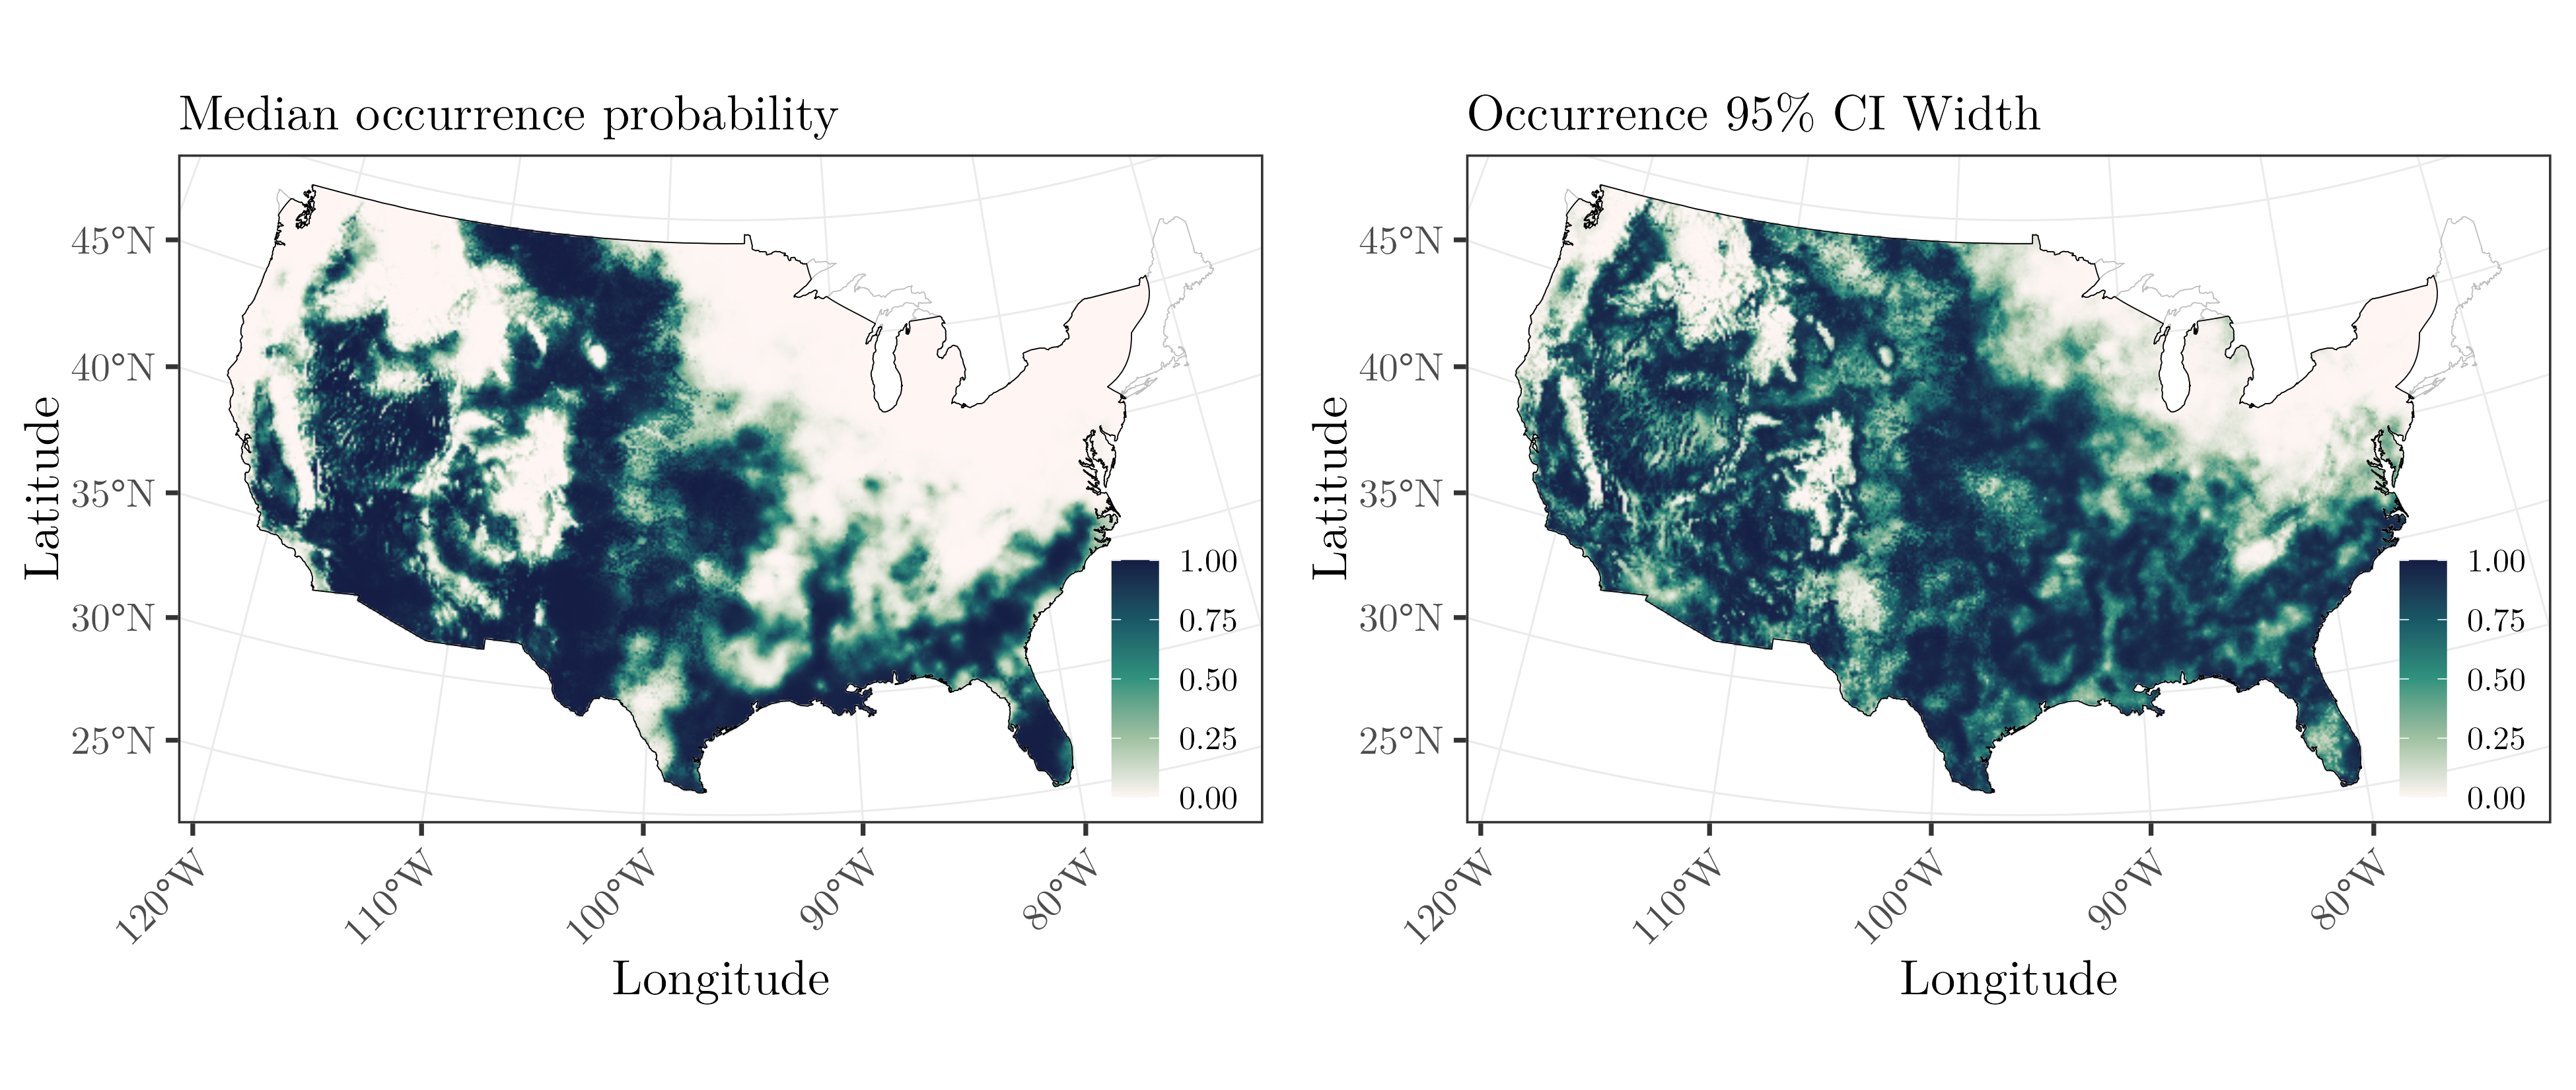
\includegraphics[scale=0.35, trim={0 1cm 1cm 2cm}, clip]{../figures/LOSH-plot.png}
          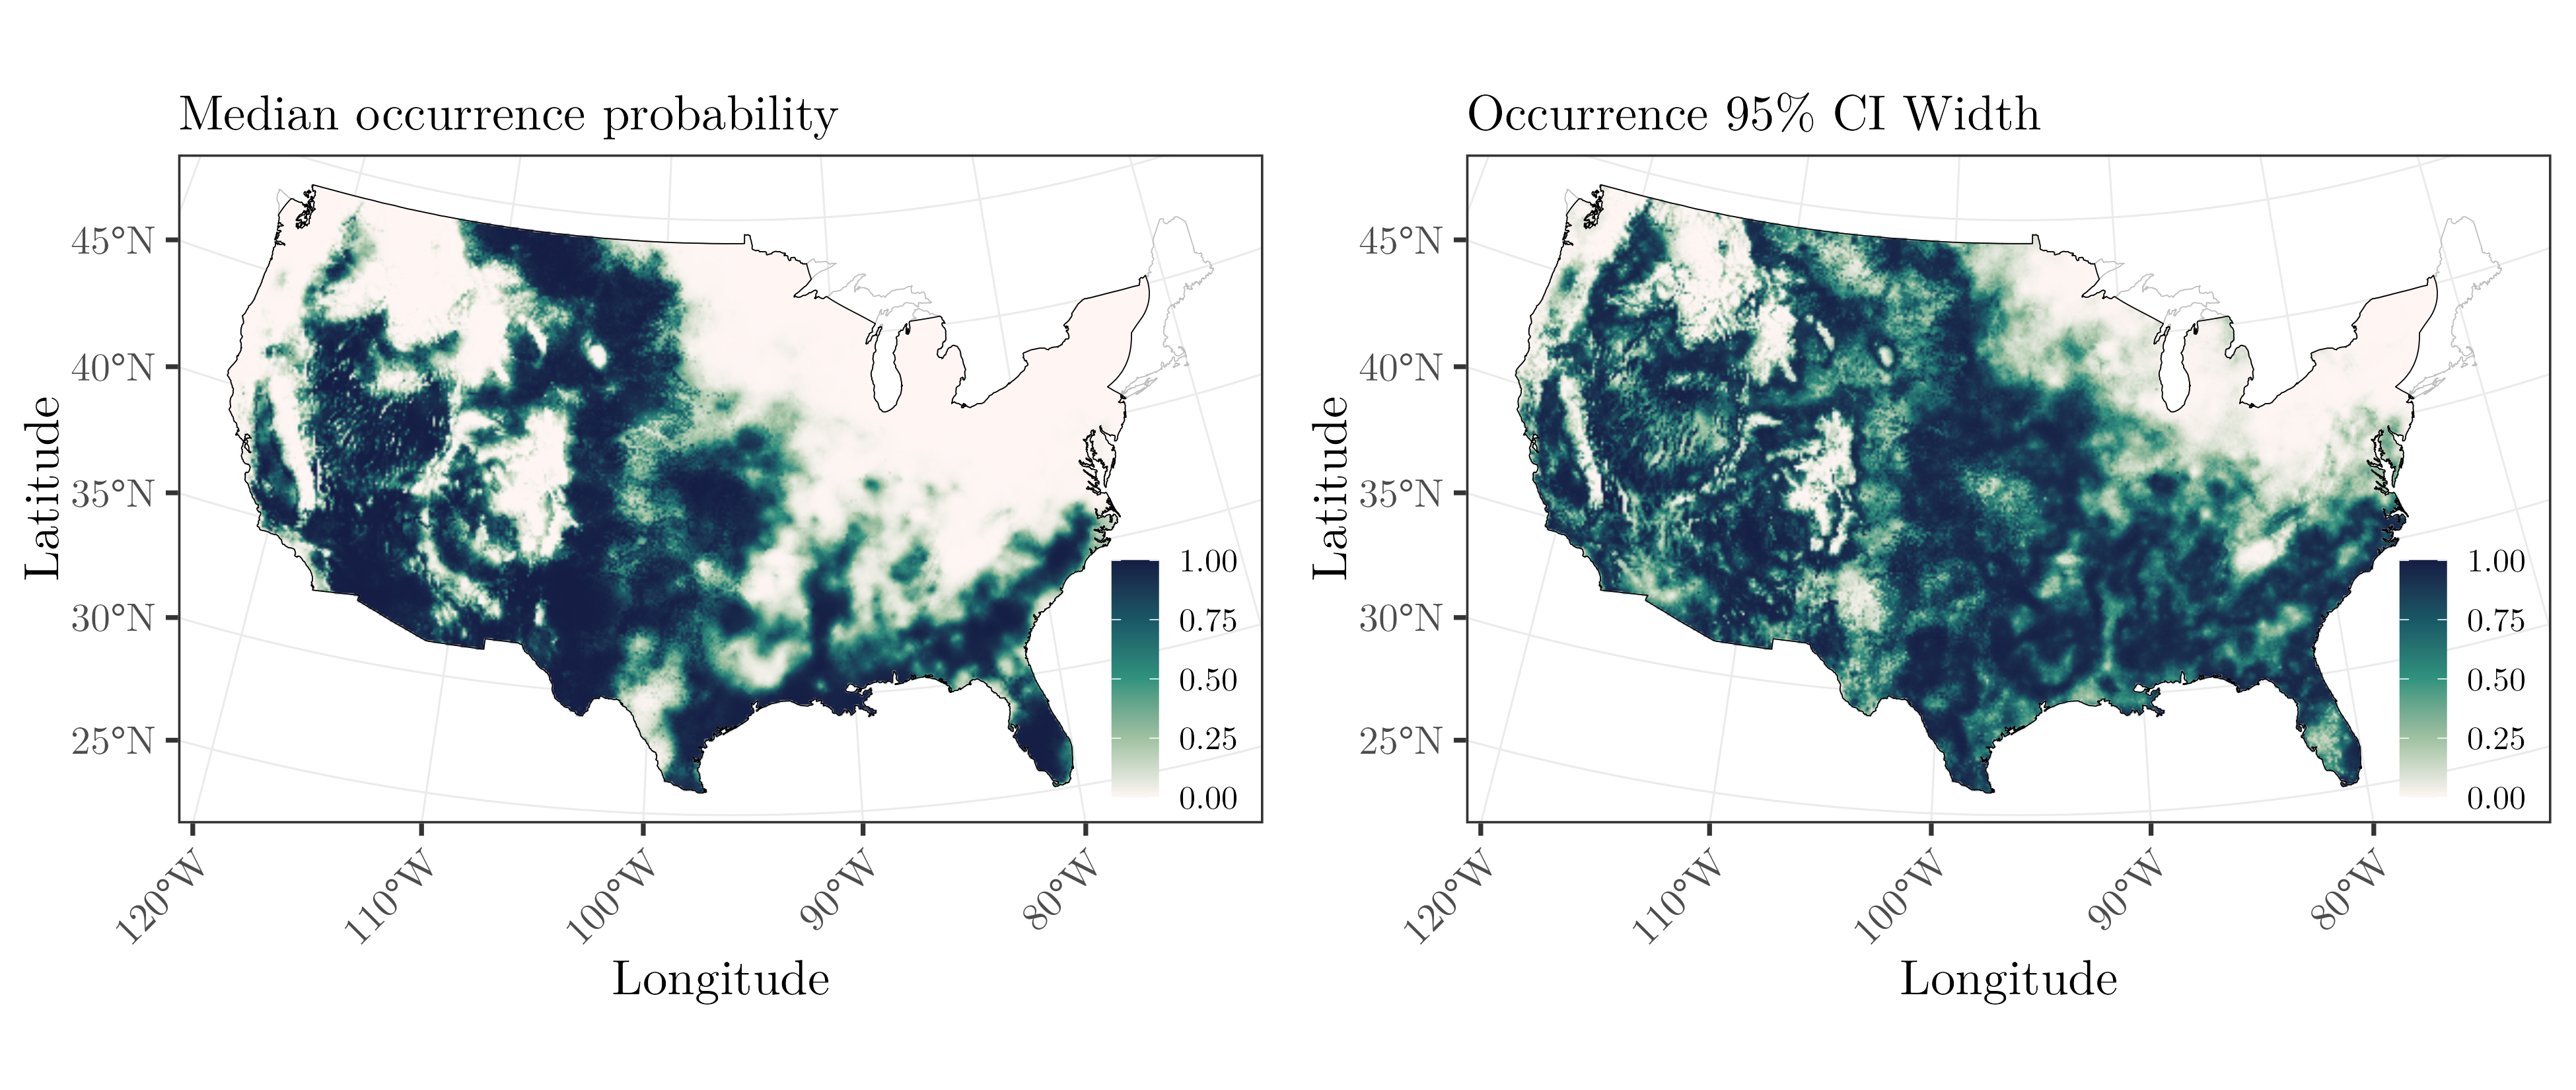
\includegraphics[width=11cm]{../figures/LOSH-plot.png}
     \end{center}

\end{frame}

\begin{frame}{Some practical considerations}
     \begin{itemize}
          \item Priors for $\sigma^2$ and $\phi$ may need to be more informative, particularly for binary data. 
	  \item Be careful with non-identity link functions when thinking about priors.
	  \item \pg data augmentation works really for binomial data. Computational cost increases as Binomial weights increases.
	  \item \pg data augmentation also applicable for Negative Binomial count data, but slow for large counts and can be unstable.
     \end{itemize}

\end{frame}
 
\begin{frame}{Software}
     \begin{itemize}
          \item \texttt{spBayes}
               \begin{itemize}
		    \item Univariate and multivariate, full GPs or predictive processes 
                    \item Gaussian, Binomial (no \pg data augmentation), Poisson
	       \end{itemize}
       \item \texttt{spNNGP} 
	       \begin{itemize}
                    \item Univariate, NNGPs
		    \item Gaussian, Binomial
	       \end{itemize}
       \item \texttt{spOccupancy}
	       \begin{itemize}
                    \item Univariate and multivariate, focus on modeling wildlife distributions, full GPs or NNGPs
		    \item Bernoulli
	       \end{itemize}
       \item \texttt{spAbundance}  (\url{https://github.com/doserjef/spAbundance})
	       \begin{itemize}
                    \item Univariate and multivariate, focus on modeling wildlife/plant abundance, NNGPs
		    \item Gaussian, Poisson, Negative Binomial
	       \end{itemize}
     \end{itemize}
\end{frame}
 
\end{document}
